\section{Measurement Techniques}
Visible light has frequencies in the THz range which is well beyond the capabilites of modern electronics to directly measure so a number of clever strategies have been developed to measure the spectral quality of laser systems.
The performance of \gls*{ps} and \gls{pdh} frequency stabilisation has been characterised using a number of methods which are detailed here.
Spectral linewidth is the principle metric by which stabilisation techniques are compared and it can be considered over a range of timescales with different implications.
Short timescales measurements, less than a second, indicate the narrowness of the frequency spectrum and are useful when considering frequency dependent interactions, such as those with atoms or optical cavities.
Long timescale measurements, minutes to hours, are useful to determine the stability of the laser and its succeptability to frequency drift and the robustness of the locking scheme.

\subsection{Heterodyne Methods}

Heterodyning is a technique, invented by Canadian Reginald Feessenden in 1901, which mixes two frequencies to produce a new frequency~\cite{cooper_physics_2001}.
The technique can be used to examine the spectral properties of lasers as the newly produced frequencies can be tailored such that they are easily measurable by photodetectors and spectrum analysers.

Laser frequency spectrum measurements using heterodyne technique are simple to implement with the correct equipment.
The two laser beams are combined such that they copropagate, requiring some mirrors and a beamsplitter/combiner, and then focussed onto a high-bandwidth photodetector, where the bandwidth is dependent on the desired resolution.
The signal from the detector can then be fed into an equally high bandwidth spectrum analyser which will display the frequency spectrum of the intensity of the light on the detector.

\subsubsection{Basic Theory}
In the electrical signals context heterodyning involves the `mixing' or multiplying of two signals (e.g. two sine waves) to produce two different signals with frequencies equal to the difference and sum of the original frequencies:
\begin{equation}
\sin(\theta_1)\sin(\theta_2) = \frac{1}{2} \cos(\theta_1-\theta_2) - \frac{1}{2} \cos(\theta_1+\theta_2).
\end{equation}

In the optical context this is achieved due to the interference term accrued when squaring the electric field in order to calculate the intensity detected by the photodetector. The intensity of an electric field is given by:
\begin{equation}
I(t) = \frac{c\epsilon_0}{2}|E|^2.
\end{equation}

For two copropagating lasers with electric fields $E_{1, 2}$ and angular frequencies $\omega_{1, 2}$ we can write
\begin{equation}
E_{i}(t) = \sin(\omega_{i}t).
\end{equation}
The electric field at the detector, $E_T$, is given by the sum of $E_{1}$ and $E_{2}$, and thus the intensity is given by,
\begin{align}
I(t) &= |E_1(t) + E_2(t)|^2\nonumber\\
&= |E_1(t)|^2 + E_1(t)E_2^*(t) + |E_2(t)|^2.
\end{align}
The interference term, $E_1(t)E_2(t)$, allows for the spectral measurements with optical signals as
\begin{align}
E_1(t)E_2(t) &= \sin(\omega_1 t) \sin(\omega_2 t) \notag \\
&= \frac{1}{2} (\cos([\omega_1-\omega_2]t) - \cos([\omega_1+\omega_2]t)), \label{equation:hetero}
\end{align}
and if $\omega_{1,2}$ are appropriately selected then the first term in Equation~\ref{equation:hetero} is measurable.
The difference in frequency ideally should be fairly small, less than a few GHz, which can often be induced on lasers with the same frequency by \glspl{aom} or \glspl{eom}.

The equations presented above provide an obviously na\"ive approach as the frequency spread of the lasers is non-zero but gives a sufficient demonstration of the basis of the heterodyne method.
The spectral profile of the heterodyne signal is formed by the convolution of the spectral profiles of the component lasers, thus if one laser is very narrow in width compared to the other then the heterodyne signal's spectral profile is approximately equal to that of the larger linewidth laser.

\subsubsection{Optical Heterodyne Methods}

There are a number of permutations of linewidth measurement techniques that utilise heterodyning. The major ones are:
\begin{itemize}
\item Heterodyne beatnote with two `identical' lasers,
\item Heterodyne beatnote between laser of interest and a relatively narrow reference laser,
\item Self-heterodyne beatnote of a laser with itself, and
\item The three-cornered hat method.
\end{itemize}


\subsubsection{Frequency Reference}

In some circumstances a second laser with a frequency linewidth much smaller than that of the laser of interest can be used to generate the heterodyne beatnote.

\subsubsection{Two-Laser Heterodyne}

Two almost identical lasers setups can be heterodyned to give the linewidth with the assumption that the lineshapes are identical.
As the lasers will be locked to the same frequency the difference in frequencies detected by the heterodyne method will the zero and spectrum analysers do not function well at zero so one of the lasers is usually frequency shifted by an \gls{aom} such that the combined lineshape of the two lasers is centred about shifted frequency.

\subsubsection{Self-heterodyne}
{\color{red}Figure}

The self-heterodyne technique involves beating a laser with itself in order to perform a heterodyne measurement\cite{okoshi_novel_1980, richter_linewidth_1986}.
The laser output is split and one portion is delayed, by $\tau_d$, by passing it through a kilometres long fibre.
The $\tau_d$ should be as long as feasible, compared to the coherence time of the laser, in order to ensure that the beams at the heterodyne detector are uncorrelated.
The remaining correlated portions of the beams result in a delta-function like peak in the frequency spectrum of the beatnote.

These are the results I got...

They look good... too good.

Here's why...\cite{richter_linewidth_1986}

\subsubsection{Three-cornered Hat}

\subsubsection{Linewidth Discrepancies}
{\color{red}I'm not certain enough about what's going on here so just remove this.}

There is an interesting discrepancy between intuition and what the literature uses to describe `linewidth'.
Intuitively, when discussing the spectral properties of light, one would expect references to refer to the properties of the electric field since that is the entity that is interacting with atoms and other frequency references.
However, the literature seems to exclusively refer to properties of the power of the signal from photodetectors, as shown on spectrum analysers, which differ by a factor of 2 which will be shown below.
Despite this fact this document follows the convention to avoid confusion.

The simplest way to examine a heterodyne signal is to look at the signal from the detector on a radio-frequency spectrum analyser.
A spectrum analyser shows the power for each frequency component of the input electrical signal.
The power of the electrical signal from the detector, $P_{elec}$ is roughly:
\begin{equation}
P_{elec}\propto I^2 \propto E^2
\label{eq:beatnote_proportional}
\end{equation}
where $I$ is the light intensity incident on the detector and $E$ is the electric field incident on the detector.

Of primary interest are the spectral properties of these signals which are given by their Fourier transform.
However we cannot simply write
\begin{equation}
\mathcal{F}[P_{elec}]\propto \mathcal{F}[I^2] \propto \mathcal{F}[E^2]
\end{equation}
since it's not true.
The inverse convolution theorem, however, can be used
\begin{equation}
f\cdot g = \mathcal{F}^{-1} \bigg[ \mathcal{F}[f] \otimes\mathcal{F}[g]\bigg].
\end{equation}

So Equation~\ref{eq:beatnote_proportional} in Fourier space becomes
\begin{align}
\mathcal{F}[P_{elec}]&\propto \mathcal{F}[I]\otimes\mathcal{F}[I]\nonumber\\
&\propto \big\{\mathcal{F}[E] \otimes\mathcal{F}[E]\big\} \otimes\big\{\mathcal{F}[E] \otimes\mathcal{F}[E]\big\}
\end{align}

For a Gaussian lineshape beatnote with \gls{rms} width $\sigma$, we can write
\begin{equation}
\mathcal{F}[E] = A e^{-(f-f_0)^2/2\sigma^2}.
\end{equation}

It is easy to show that the convolution of two Gaussians produces another Gaussian with variance equal to the sum of the variance of the two constituent functions.
Thus,
\begin{equation}
\mathcal{F}[I] = B e^{-(f-f_0)^2/4\sigma^2}
\end{equation}
and
\begin{align}
\mathcal{F}[P] &= B e^{-(f-f_0)^2/8\sigma^2}\nonumber\\
&= B e^{-(f-f_0)^2/2(2\sigma)^2}
\end{align}
So the width of the signal shown on a spectrum analyser has twice the spectral width of the electric field that generated it.

\begin{figure}
\centering
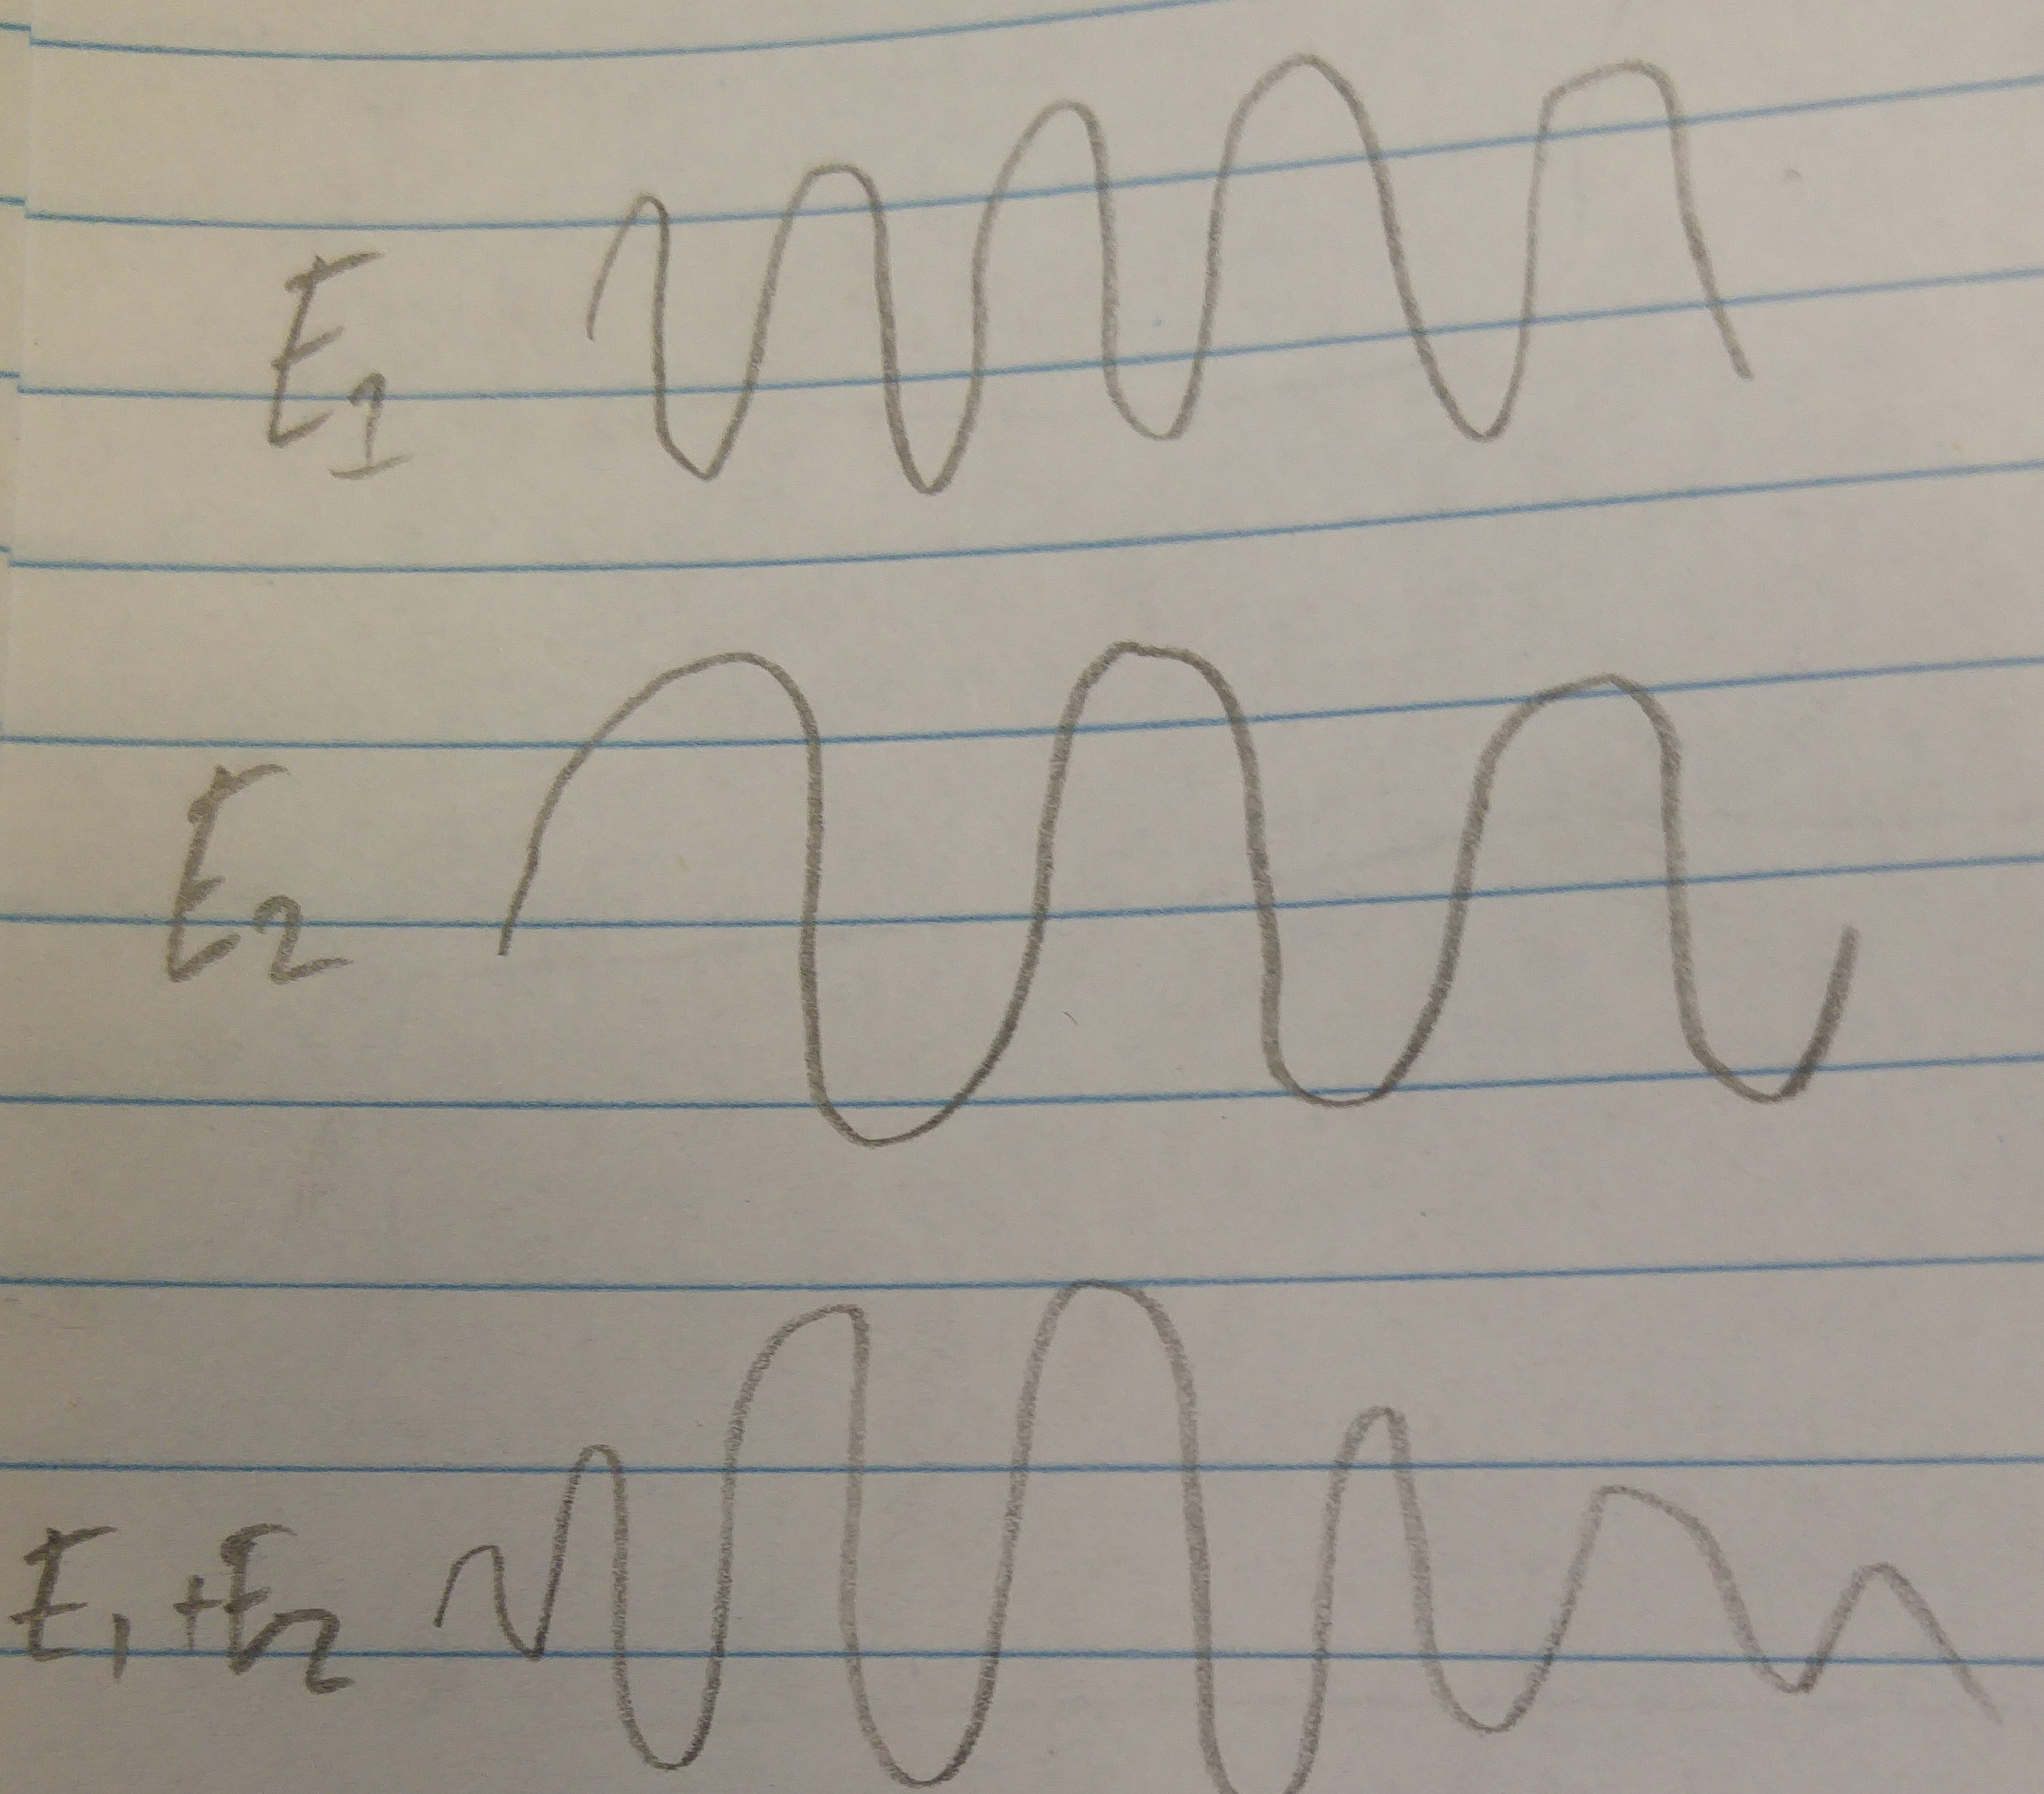
\includegraphics[width=0.5\linewidth]{part1/Figs/beatnote.jpg}
\caption{Depiction of simple beatnote.}
\label{figure:simple_beatnote}
\end{figure}


\subsection{cavity Measurements}

\subsubsection{Two-Sided Peak Measurements}

\subsubsection{One_Sided Peak Measurements}

\subsection{Noise measurements}

\subsubsection{Bandwidth Stuff}

\subsubsection{Noise Integration}

\subsection{Long Term Stability}

